\documentclass{ximera}

\begin{document}
    \author{Wim Obbels}
    \xmtitle{Ximera Demo}{Een eenvoudige Ximera module}
    \label{xim:ximeraDemo}

Dit document bevat een bondig overzicht van enkele mogelijkheden van Ximera. 

% Demo over het toch-niet-helemaal-gelijk makken van PDF en HTML ... !
\pdfOnly{
    \ifhandout
    Je gebruikt de HANDOUT PDF versie van deze demo.
    
    Er bestaat ook een \textit{standaard} PDF \textit{die antwoorden en hints bevat}.
    \else
    Je gebruikt de STANDAARD PDF versie van de demo; 

    Er bestaat ook een \textit{handout} PDF \textit{zonder de antwoorden}.
    \fi
    
    Er bestaat ook een  \textit{online} versie met extra functionaliteit.
    
}

\begin{onlineOnly}
    Je gebruikt de ONLINE versie van de demo; onderaan kan je een PDF versie downloaden waar een licht andere inleiding staat. In de PDF versie wordt verwezen naar het bestaan van deze online versie.
\end{onlineOnly}


\section{Oefeningen en interactieve inhoud}\label{sec:demo:voorbeelden_problemen}
\begin{exercise}    
    Los volgende invulvragen correct op:
    \begin{question}
        $1+1 = \answer{2}$\label{itm:showCase:voorbeeld_answer}    
    \end{question}
%    \begin{question}
%        $1+1 = \answer[given]{2}$ 
%        
%        Met 'answer[given]' is het antwoord is ook beschikbaar in de handout, en in de standaard PDF staat er een extra blokje rond, zodat het opvalt)
%    \end{question}
    \begin{question}
         $\frac{1}{2} =  \answer{\frac{1}{2}}$  
         % $\frac{1}{2} =  \answer{0.5}$     werkt natuurlijk ook
         
         \begin{onlineOnly}
         Gebruik een \textit{punt} voor decimale getallen, en/of een breukstreep of \textit{\textbackslash frac} voor breuken ...
         \end{onlineOnly}
         
%         Gebruik in \LaTeX in \verb|\answer| enkel  \verb|\frac| voor breuken (en geen \verb|\dfrac|...) 
    \end{question}
    \begin{question}
        $\frac{1}{3} =  \answer[tolerance=.02]{0.33}$  
        
        Een auteur kan een nauwkeurigheid opgeven. Hier mag er 0.02 naast zitten.
    \end{question}
\end{exercise}

\begin{exercise}
       Los volgende meerkeuzevragen correct op:
    \begin{question}
        $1+1 = $\wordChoice{\choice[correct]{$2$}\choice{$3$}\choice{geen van de eerste twee opties}\choice{de derde optie}}
        
        Online is er een dropdown, in de PDF één lijn met een lijst van (hopelijk erg bondige) mogelijkheden.
        %Eenvoudige \verb|\wordchoice| wordt dropdown in HTML.
    \end{question}
    \begin{question}
        $1+1 = $\begin{multipleChoice} \choice[correct]{$2$}\choice{$3$}\choice[correct]{$3-1$}\choice{geen van de vorige antwoorden}\choice{het bovenstaande antwoord}\end{multipleChoice}
        
        Meerkeuze waarbij meerdere mogelijkheden correct kunnen zijn, het volstaat er één aan te duiden.
        %Eenvoudige \verb|\begin{multipleChoice}| wordt tabel in HTML met maximaal één keuzemogelijkheid. Er kunnen meerdere correcte antwoorden zijn.
        
    \end{question}
    \begin{question} 
        $1+1 = $\begin{selectAll} \choice[correct]{$2$}\choice{$3$}\choice[correct]{$3-1$}\choice{geen van de vorige antwoorden}\choice{het bovenstaande antwoord}\end{selectAll}
    
        Meerkeuze waarbij meerdere mogelijkheden correct kunnen zijn, en alle correcte antwoorden moeten worden aangeduid.
%        Eenvoudige \verb|\begin{selectAll}| wordt tabel in HTML waarbij alle correcte keuzes moeten worden aangeduid.    
    \end{question}
    
\end{exercise}

\begin{exercise}
    Los volgende vragen correct op. 
    
    Er zijn telkens hints en/of feedback.
    
        \begin{question} % (Gebruik de hint!)
          $2+2 = $\wordChoice{\choice{$2$}\choice{$3$}\choice[correct]{$4$}\choice{geen van de vorige antwoorden}\choice{het vorige antwoord}}
          \begin{hint}
              Per definitie is $2 = 1+1$, en de optelling associatief.
           \end{hint}  
           \begin{hint}
              Voor $1+1+1+1$ hebben we een kortere notatie ingevoerd.
           \end{hint}
           \begin{feedback}[correct] 
              Proficiat, je kan al erg goed rekenen! Doe zo voort. 
              Deze feedback verschijnt enkel bij een correct antwoord.
           \end{feedback}          
        \end{question}
   
        \begin{question}
          Als $y=4+4$ dan is $y = \answer[format=integer,id=y]{8}$ 
          
          Het antwoord is een geheel getal, maar probeer eerst bijvoorbeeld $4.4$, en dan een fout geheel getal, bijvoorbeeld $7$.)
          \begin{hint}[0]
              Heb je 7 al geprobeerd (want dan krijg je erg nuttige feedback!)
          \end{hint}
          \begin{hint}
            Herbekijk het antwoord van de vorige vraag voor de precieze betekenis van het symbool $4$ !
          \end{hint}
          \begin{hint}[3]
            Dit is gewoon een elementaire optelling, ja ....
          \end{hint}
      
          \begin{feedback}[correct]
              Correct !
          \end{feedback}
%          \begin{feedback}[y<>8]
%               Fout !
%           \end{feedback}
          \begin{feedback}[attempt]
            De organisatie laat niet na u bij deze vriendelijk te danken voor uw verdienstelijke poging om deze vraag te beantwoorden.
            
            (Deze feedback met \verb|[attempt]| verschijnt bij elke antwoordpoging.)   
           \end{feedback}
      
          \begin{feedback}[y==7]
            Wel, je volgt de richtlijnen erg nauwkeurig. Maar ook voor andere foute antwoorden geven we interessante feedback.
            
            (Deze feedback met \verb|[y==7]| verschijnt enkel bij antwoordpoging met antwoord $7$.)   
            
          \end{feedback}
          \begin{feedback}[y==8]
          Proficiat. Je heheerst deze module voldoende. Je bent nu uitstekend voorbereid om verder te gaan naar de fascinerende problematiek van \link[HoTT]{https://github.com/HoTT/HoTT}

          (Deze feedback met \verb|[y==8]| verschijnt enkel bij het correcte antwoord.)   

          \end{feedback}
          \begin{feedback}[y<7]
              Mmm, dat is wat weinig. Reken alles nog eens nauwkeurig na.
              
              (Deze feedback met \verb|[y<7]| verschijnt enkel bij een te klein antwoord.)   
            \end{feedback}
          \begin{feedback}[y>8]
               Mmm, dat is wat veel. Reken alles nog eens nauwkeurig na.

              (Deze feedback met \verb|[y>7]| verschijnt enkel bij een te groot antwoord.)   

           \end{feedback}
       \end{question}

	\begin{question}
		Sommige antwoorden zijn te moeilijk om te laten intypen, en dan toont \verb|\answer[onlinenoinput]| enkel een knop 'Toon Antwoord':
        
        Schrijf met een sommatie de som van de vierkantswortels van de getallen 1 tot en met $100$ telkens tot de macht $\log 2$:  $\answer[onlinenoinput]{\sum_x^{x=100}(\sqrt{x^{\log 2})}}$
        
        % todo: investigate ;-)
        %(Pas op:  op 23/11/2020 werkte dit \textsc{niet}.)  ???
		\begin{oplossing}
			Hier komt dan een uitwerking van de oefening.
		\end{oplossing}
	\end{question}
	\begin{question}
		Soms kunnen antwoorden wel worden ingegeven, maar het is niet perse nuttig, en dan toont  \verb|\answer[onlineshowanswerbutton]| een extra sleuteltje om het juiste antwoord te tonen:
        
        Schrijf de vierkantswortel van $x$-tot-de-macht-$\log 2$ ?  $\answer[onlineshowanswerbutton]{\sqrt{x^{\log 2}}}$
		\begin{oplossing}[toon]
			Hier komt dan een uitwerking van de oefening.
		\end{oplossing}
	\end{question}
\end{exercise}


\section{Integratie met andere omgevingen}

Volgend youtube filmpje geeft een korte inleiding tot de goniometrie:
\begin{center}
 \youtube{2jGHOcxB8sI}
\end{center}


maar je kan ook zelf experimenteren met een interactieve grafiek van de cosinus met Desmos:

\[  
\graph[xmin=-5,xmax=20,ymin=-1,ymax=1]{y=cos(x)}  
\] 

\pdfOnly{
     (Omdat u de PDF versie gebruikt, tonen we hier enkel een eerder \textit{saaie} grafiek met tikz: )
    
\begin{image}[\textwidth]
    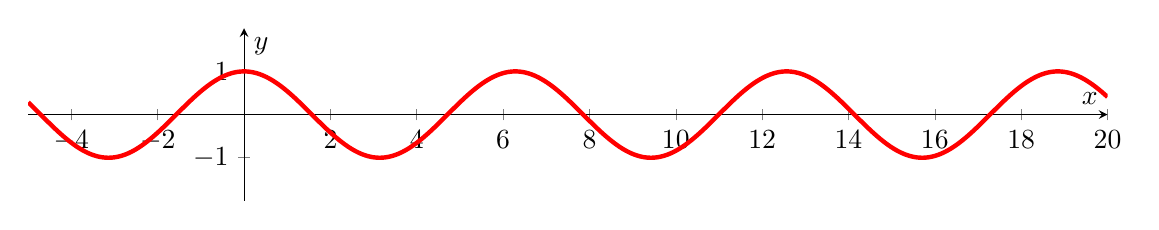
\begin{tikzpicture}
    \begin{axis}[
    scale=2,
    axis equal image,
    samples=500,
    axis lines=middle,
    ymin=-2,ymax=2,
    ytick={-1,1},
    ylabel=$y$, 
    xlabel=$x$
    ]
    \addplot[domain=-5:20, black, ultra thick, color=red] {cos(deg(x))};
    \end{axis}
    \end{tikzpicture}
\end{image}
}

of met de eigenschappen van drie rechten in Geogebra:
%todo: betere geobegra applet kiezen ...

\begin{center}
    \geogebra{zwrge8pa}{800}{800}
\end{center}



\section{Environments en styling}

\subsection{Voorbeelden van het gebruik van environments}

Er is een lijst van environments die een aangepaste (en aanpasbare) formattering hebben, en in het geval van oefeningen ook een speciale functionaliteit.

\begin{definition}[Absolute waarde]\label{showcase:absolutewaarde}
	Voor een reëel getal $a\in\R$ definiëren we de \textit{absolute waarde} van $a$, genoteerd $|a|$, als
	\[
		|a| \perdef\displaystyle\ 
		          \left\{
			\begin{array}{rll  } 
				a  & \mbox{als} & a \geq 0 \\
				-a & \mbox{als} & a<0.
			\end{array}\right.
	\]
\end{definition}
\begin{remark}[Eigenschappen van de absolute waarde (met $a\in\R$)] \nl
		\begin{enumerate}
			\item Pas op: $|-a|= |a|$, maar \textsc{zeer zeker niet} $\xcancel{|-a|=a}$
			
			$|-a|=a$ is \textsc{fout} als $a<0$: als $a=-7$, dan is $|-a| = |-(-7)| \neq -7 = a$
			\item $|a^2 + 1| = a^2 + 1$, want $a^2+1$ is altijd positief.
			\item $|a^2 - 1| = ....$ \qquad(er is \textsc{geen} eenvoudige algemene formule zonder $|\cdot|$)
\end{enumerate}
\end{remark}
\begin{example}[Eenvoudige voorbeelden van absolute waarden] \nl 
	
\begin{xmmulticols}
		\begin{enumerate}
			\item $|5|=5$ en $|-5|=5$
			\item $|2 + 1| = |2| + | 1|\quad (=3)$
			\item $|2 + (-1)| \neq |2| + | -1|$ (want $1\neq 3$)
			\item $|(-3)^2| = |3^2| = 9\quad (=|-3^2| = |-9|) $ 
			
			\item $|\sqrt{2}-1|=$\wordChoice{\choice[correct]{$\sqrt{2} - 1$}\choice{$1-\sqrt{2}$}}
			\item $|1-\sqrt{2}| = $\wordChoice{\choice[correct]{$\sqrt{2} - 1$}\choice{$1-\sqrt{2}$}}
			\item $|2-\sqrt{2}| = $\wordChoice{\choice{$\sqrt{2} - 2$}\choice[correct]{$2-\sqrt{2}$}}
			\item $|\sqrt{2}-2| = $\wordChoice{\choice{$\sqrt{2} - 2$}\choice[correct]{$2-\sqrt{2}$}}			
		\end{enumerate}
\end{xmmulticols}
\end{example}

In de pdf kan de stijl worden aangepast via alle standaard LaTeX mogelijkheden. Voor de online versie bestaat de mogelijkheid zelf css files toe te voegen:
	\begin{itemize}
		\item \verb|global.css| in de root map van de repository: alle modules in de repository gebruiken deze styling
		\item \verb|xoursefilename.css| in de folder van xoursefilename.tex file: alle modules in de xourse gebruiken deze styling
		\item \verb|activityfilename.css| in de folder van de activityfilename.tex file: styling specifiek voor 1 activity.
	\end{itemize}
%	De \verb|ximeraShowcase.css| file specifieert in dit geval dat de questions niet alleen links maar ook rechts een paarse balk hebben. 
    % niet het geval ...?



\end{document}
